\documentclass[tikz,border=2pt]{standalone}
\usepackage{amsmath,amssymb}
\usepackage{tikz}
\usetikzlibrary{arrows.meta}

\begin{document}
% A bounded set fits inside one ball B(x0, M): no point of E is further than M from x0.
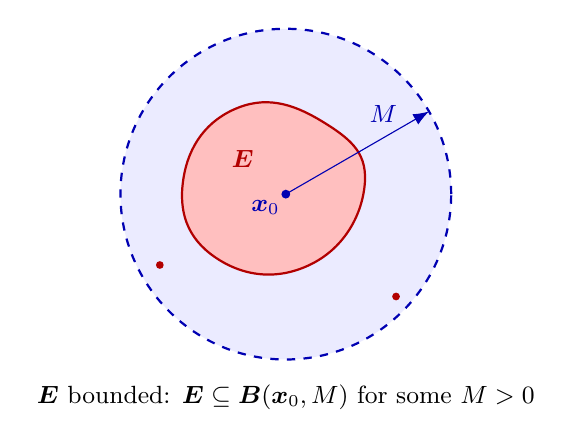
\begin{tikzpicture}[every node/.style={font=\small}]
	\fill[blue!8] (0,0) circle (2.1);
	\draw[blue!70!black, thick, dashed] (0,0) circle (2.1);
	\fill[red!25] plot[smooth cycle, tension=0.8] coordinates {(-1.3,0.2) (-0.6,1.1) (0.5,0.9) (1.0,0.1) (0.3,-0.9) (-0.9,-0.8)};
	\draw[red!70!black, thick] plot[smooth cycle, tension=0.8] coordinates {(-1.3,0.2) (-0.6,1.1) (0.5,0.9) (1.0,0.1) (0.3,-0.9) (-0.9,-0.8)};
	\node[red!70!black] at (-0.55,0.45) {$\boldsymbol{E}$};
	\fill[red!70!black] (1.4,-1.3) circle (1.4pt);
	\fill[red!70!black] (-1.6,-0.9) circle (1.4pt);
	\draw[-{Latex[length=2mm]}, blue!70!black] (0,0) -- (30:2.1);
	\fill[blue!70!black] (0,0) circle (1.6pt);
	\node[blue!70!black, below left, inner sep=2pt] at (0,0) {$\boldsymbol{x}_0$};
	\node[blue!70!black, above left, inner sep=1.5pt] at (30:1.7) {$M$};
	\node[anchor=north] at (0,-2.3) {$\boldsymbol{E}$ bounded: $\boldsymbol{E}\subseteq\boldsymbol{B}(\boldsymbol{x}_0,M)$ for some $M>0$};
\end{tikzpicture}
\end{document}
